\documentclass[a4paper, 12pt]{article}
\usepackage{mathptmx}
\usepackage[utf8x]{inputenc}
\usepackage{amsmath}
\usepackage{graphicx}
\usepackage[margin=2cm]{geometry}
\DeclareSymbolFont{extraup}{U}{zavm}{m}{n}
\DeclareMathSymbol{\varheart}{\mathalpha}{extraup}{86}
\DeclareMathSymbol{\vardiamond}{\mathalpha}{extraup}{87}
\usepackage{nameref, hyperref}
\usepackage{float}
\usepackage{cite}
\setlength{\parskip}{1em}
\bibliographystyle{plos2015}


\begin{document}

\begin{flushleft}
{\Large
\textbf\newline{\textit{CorShrink}: A random multi-target adaptive shrinkage method for correlation matrix estimation} 
}

Kushal K Dey \\
University of Chicago, Dept. of Statistics, \\
5220 S Kenwood Ave, \\
Chicago, IL, 60615 \\
\end{flushleft}

\begin{center}
\textbf{Abstract} \\ \vspace{0.2 in}
\end{center}
\begin{flushleft}
{\small Shrinkage estimation of correlation matrices provides well conditioned and more accurate estimators of the population correlation matrix, specially in `small n, large p` contexts. In this paper, we propose a multi target shrinkage method called \textit{CorShrink} where the targets are noisy versions of identity matrix and which learns adaptively the optimal amount of shrinkage from the data. We compare the performance of our method under different $(n,p)$ scenarios with respect to the standard approaches and also provides a demonstration of the performance of our approach on a single cell RNA-seq data from mouse pre-implantation and we show the method indeed extracts useful biological features from the data. The methods are implemented in a Github R package \textbf{CorShrink}. } \\ \vspace{0.2 in}

\textbf{Keywords}: shrinkage, covariance matrix estimation, variational EM, single cell RNA-seq
\end{flushleft}

\normalsize

\section{Introduction}
Estimation the covariance or correlation matrix of the variables is a common practice for researchers interested in a broad spectrum of statistical applications, ranging from understanding the relationship among variables, perform classification or regression and even form groups or clusters or features. The most common choice of an estimator is the sample covariance or correlation matrix which is also the Maximum Likelihood estimate. While this estimator works fine for $ n > p$ cases, it has extremely high approximation error with respect to the population covariance/correlation matrix due to its low rank structure when $ n << p$. 

In 2003, Ledoit and Wolf proposed an estimator that is well conditioned and has much lesser approximation error than the sample correlation matrix \cite{Ledoit2003} \cite{Ledoit2004} in particular under $n <<p$ scenarios. This approach was further developed and generalized by Sch\"{a}fer and Strimmer, who besides proposing new shrinkage estimators, also provided  analytic calculation of the optimal shrinkage intensity \cite{Shafer2005}. The idea was to fit a convex combination of the empirical sample covariance matrix (S) along with a chosen target matrix T, which can be chosen to be an  identity matrix or constant correlation matrix. The mixing proportion $\delta$ in the convex combination $\delta T + (1- \delta) S$ is usually selected to minimize the expected error of approximation of the shrunken estimate. The above papers used a single target for shrinking, but a multi-target covariance shrinkage approach was recently proposed - see Lancewicki and Aladjem  2014 \cite{Lancewiki2014}. 

In this paper, we propose three versions of an alternative method called \textit{CorShrink} which assumes multiple targets 
$T_1$, $T_2$, $\cdots$, $T_K$, all of which are noisy versions of the identity matrix and the noise variation increases with each $k$. We adaptively determine the amount of shrinkage by optimally determining the shrinkage weights for each target and assuming that the set of targets cover the range of variation of the data well. We will discuss about the noise structure and the model fit in more details in the Methods section.  We also perform comparisons of our model performance with respect to the Sch\"{a}fer and Strimmer approach and the Graphical LASSO algorithm developed by Friedman et al \cite{Friedman2008} for sparse representation of the correlation and primarily inverse correlation matrices used for building causal networks. We show that  \textit{CorShrink} performs marginally better than the Sch\"{a}fer and Strimmer shrinkage in terms of eigenspace approximation to the population covariance when $ n << p$, and both \textit{CorShrink} and Shafer-Strimmer method perform much better as correlation shrinkage methods compared to GLASSO. We also show an application our method on a single cell mouse pre-implantation RNA-seq data due to Deng et al. 2014 \cite{Deng2014}.



\section{Methods and Materials}

As a simple version of a shrinkage estimator for a covariance matrix, one fits a convex combination of the empirical sample covariance matrix (S) along with a chosen target matrix T, which can be chosen to be an  identity matrix or constant correlation matrix. The mixing proportion $\delta$ in the convex combination $\delta T + (1- \delta) S$ is usually selected to maximize the expected accuracy of the shrunken estimator. In our approach, we shrink the correlations to $0$, implying the target matrix is the identity matrix. However, instead of a single target $T$, we assume multiple random targets $T_1$, $T_2$, $\cdots$, $T_k$, all centered around the same identity correlation matrix but each with different degrees of noise variation, usually increasing with $k$. The belief is that such an approach would adaptively decide on the amount of shrinkage without requiring to follow a Cross Validation approach. 

Let us denote the sample correlation matrix by $R = ((r_{ij}))_{i, j = 1,2, \cdots, P} $, $P$ being the number of features, calculated over $N$ data samples.

\begin{equation}
r_{ij} = \frac{s_{ij}}{\sqrt{s_{ii} s_{jj}}}   \hspace{1 in} s_{ij} = \frac{1}{n} \sum_{n=1}^{N} \left ( x_{ni} - \bar{x}_{i} \right ) \left ( x_{nj} - \bar{x}_{j} \right ) 
\end{equation}

where $s_{ij}$ is the sample covariance between the vectors $x_{*,i}$ and $x_{*,j}$.

We propose the following model

For any two features $i$ and $j$ with $ i < j$ , we define a binary size K latent variable vector $((Z_{ij:k}))$  where $Z_{ij:k}$ takes the values $1$ with probability $\pi_{k}$ and $0$ otherwise. 

%$$  Pr \left [ Z_{ij:k} = 1  \right ] = \pi_{k}    \hspace{1 in}  j < i $$

\begin{equation}
Pr \left [ Z | \pi \right ] = \prod_{i=1}^{P} \prod_{j < i} \prod_{k=1}^{K} \pi_{k}^{Z_{ij:k}}  
\end{equation}

We define  latent variables $\rho_{ij}$, such that

\begin{equation}
Pr \left ( \rho |  Z, \pi  \right )  = \prod_{i=1}^{P} \prod_{j < i} \prod_{k=1}^{K} \left [ N \left (\rho_{ij} : 0, \sigma^2_{k} \right ) \right ]^{Z_{ij:k}}  
\end{equation}

We assume Normal distribution for the $\rho$,

\begin{equation}
Pr \left (\hat{\rho}_{ij} | \rho \right ) = \prod_{i=1}^{P} \prod_{j < i } N \left (\hat{\rho}_{ij} | \rho_{ij}, s^2_n = \frac{1}{n-3} \right)  
\end{equation}

where $\hat{\rho}_{ij}$ are the Fisher's z-scores of the sample correlations $r_{ij}$ given by 

\begin{equation}
\hat{\rho}_{ij} = \frac{1}{2} \log \left ( \frac{1+r_{ij}}{1- r_{ij}} \right ) 
\end{equation}

The model implies that we shrink the $ \hat{\rho}_{ij}$ to $0$ but the amount of shrinkage is decided both by the number of independent samples $s^2_{n} = \frac{1}{n-3}$ and also by $\sigma_{k}$. 

We propose three different models depending on our assumptions on $\pi$ and $\sigma$. 

\begin{itemize}

\item \textit{CorShrink-ML}:  We choose a fixed grid of $\sigma$ values, selected such that it covers the span of the variation of the data well. Here we propose to use a similar grid (with minor adjustments) as suggested in Stephens 2016 \cite{Stephens2016} for modeling false discovery rates. We add a component with $\sigma_k=0$ that represents the null component of the prior. We fit the mixing proportions $\pi$ of the components using EM algorithm. 

\item \textit{CorShrink-VEM}: We use the same grid of $\sigma$ values as in the \textit{CorShrink-ML} model, but now we assume a Dirichlet prior on $\pi$, that puts a high weight on the null component and treats the other components equivalently. From performance comparisons on simulated data, we assumed the default Dirichlet prior to be $Dir(10, 1, ,1, \cdots, 1)$. 

\item \textit{CorShrink-VEM2}: We additionally assume the $\sigma$ values to be not fixed but to come from a Inverse-Gamma distribution. We assume $Inv-Gamma(\epsilon, \epsilon)$ distributions which are relatively non-informative in order to make the choice of $\sigma$ very flexible. For our applications in this paper, assume $\epsilon$ to be $0.01$.

\end{itemize}

The estimation of $\pi$ for the \textit{CorShrink-ML} model was performed using the \textbf{ashr} package due to Matthew Stephens \cite{Stephens2016}, which fits an EM algorithm. For the \textit{CorShrink-VEM} and \textit{CorShrink-VEM2}, we use Mean Field Variational EM models to estimate the model parameters. Variational methods are faster than MCMC methods as they often provide analytic updates to parameters thereby ensuring faster computation \cite{Beal2003} \cite{Beli2016}.

For \textit{CorShrink-VEM2} model where $\pi$ and $\sigma$ are both random, we first perform a change of variables 

$$ \xi_{k} = \sigma^2_{k} + \frac{1}{n-3} $$

Suppose the priors on $\pi$ and $\xi$ are 

$$ \pi \sim Dir \left ( \alpha_1, \alpha_2, \cdots, \alpha_{K} \right ) \hspace{1 in} \xi_{k} \sim Inv-Gamma(a, b) \;\; \forall \; k $$

and then define the mean field variational distribution on the latent variable $Z$ and the parameters $\pi$ and $\xi_1, \xi_2, \cdots, \xi_{K}$ as follows. 

$$  q(Z, \pi, \xi) = q(Z) q(\pi) \prod_{k=1}^{K} q(\xi_{k})   $$

Then the mean field distribution for $\pi$ is given by 

\begin{align}
\log q^{\star} (\pi)  & = E_{Z, \xi} \left [   \log p (\hat{\rho}, Z, \pi, \xi ) \right ]   \\
			    & = E_{Z} \left [ \sum_{k=1}^{K} \left (\alpha_{k} - 1\right) \log (\pi_k) + \sum_{i=1}^{J} \sum_{j < i} \sum_{k=1}^{K} z_{ij:k} \log (\pi_{k} ) \right ]  + const. \\
			    & = \sum_{k=1}^{K} \left [   \left (\alpha_{k} - 1\right)  + \sum_{i=1}^{J} \sum_{j < i}  \delta_{ij:k} \right]\log (\pi_{k})  \\
\end{align}

So the variational distribution for $\pi$ is of the form 

\begin{equation}
\pi \sim Dir \left (   \pi | \beta_1, \beta_2, \cdots, \beta_{K} \right ) \hspace{1 in}   \beta_{k} = \alpha_{k} + \sum_{i=1}^{J} \sum_{j < i} \delta_{ij:k} 
\end{equation}

The variational distribution of the latent variable $Z$ is obtained similarly

\begin{align}
\log q^{\star} (Z)  & = E_{\pi, \xi} \left [  \log p ( \hat{\rho}, Z, \pi, \xi ) \right ]   \\
			  & = E_{\pi, \xi} \left [   \log p(Z | \pi) +  \log p (\hat{\rho} | Z, \xi, \pi) \right ] \\
			  & = \sum_{i=1}^{P} \sum_{j < i}  \sum_{k=1}^{K} z_{ij:k} E_{\pi} \left (  \log (\pi_{k}) \right)  + \sum_{i=1}^{P} \sum_{j < i}  \sum_{k=1}^{K} z_{ij:k}  \left [ \frac{1}{2}  E_{\xi} \left [ \log \frac{1}{\xi_{k}} \right] - \frac{\hat{\rho}^2_{ij}}{2}  E_{\xi} \left [ \frac{1}{\xi} \right ] \right] \\
\end{align}

It can be shown that 

\begin{equation}
E_{\xi_{k}} \left [ \log \frac{1}{\xi_{k}} \right]  = - \log (\nu_{2k}) + \psi(\nu_{1k})   \hspace{0.4 in} E_{\xi_{k}} \left [ \frac{1}{\xi_{k}} \right ]  = \frac{\nu_{1k}}{\nu_{2k}} \hspace{0.4in} E_{\pi} \left (  \log (\pi_{k}) \right)  = \psi (\beta_{k}) - \psi (\sum_{l=1}^{K} \beta_{l} )
\end{equation}

where $\psi$ represents the digamma function. Using all of the above results, we get the following distribution of $Z$,

\begin{equation}
 q^{\star}(Z) = \prod_{i=1}^{P} \prod_{j < i} \prod_{k=1}^{K} \delta_{ij:k}^{Z_{ij:k}} \hspace{0.4in} 
\delta_{ij:k} \propto \exp \left (   \left \{ \psi (\beta_{k}) - \psi (\sum_{l=1}^{K} \beta_{l} ) + 0.5 \times ( \psi(\nu_{1k}) - \log (\nu_{2k}) ) -  \frac{\hat{\rho}^2_{ij}}{2} \frac{\nu_{1k}}{\nu_{2k}} \right \}  \right ) 
\end{equation}


For \textit{CorShrink-VEM} model, the $\sigma_{k}$ or $\xi_{k} = \sigma_{k} + \frac{1}{n-3}$ are fixed and the variational distribution is of the form 

\begin{equation}
q(Z, \pi) = q(Z) q(\pi) 
\end{equation}

The variational distribution is same as in \textit{CorShrink-VEM2} model, whereas the variational distribution of $Z$ can be achieved similarly as follows 

\begin{equation}
 q^{\star}(Z) = \prod_{i=1}^{P} \prod_{j < i} \prod_{k=1}^{K} \delta_{ij:k}^{Z_{ij:k}}
\hspace{0.4 in} \delta_{ij:k} \propto \exp \left (   \left \{ \psi (\beta_{k}) - \psi (\sum_{l=1}^{K} \beta_{l} ) + 0.5 \times \left ( \log \frac{1}{\xi_{k}} \right ) -  \frac{\hat{\rho}^2_{ij}}{2} \frac{1}{\xi_{k}} \right \}  \right ) 
\end{equation}

The \textit{CorShrink-VEM2} model is flexible in choice of $\pi$ and $\xi_{k}$'s, however it also has the problem of hitting a local maxima and the $\sigma_{k}$'s for multiple $k$'s to converge to same point. In order to counter that, we initialize the parameters first using the  \textit{CorShrink-VEM} model that assumes a fixed grid of well spread out $\xi_{k}$ values. 
Post the initialization, we apply the \textit{CorShrink-VEM2} model to the parameters. 

The other point to note is that actually the $\xi_{k}$'s are bounded below by $\frac{1}{n-3}$ which we ignore in defining an Inverse Gamma distribution on the $\xi$. This is a compromise for very small $n$ and we do therefore do not recommend the use of \textit{CorShrink-VEM2}  for very small $n$ values. Having said that, the initialization using \textit{CorShrink-VEM} fixes the $\xi_{k}$ initial values to be $ > \frac{1}{n-3}$ and we usually find that the final estimates would automatically adjust themselves to the lower bound and in case they violate, we forcibly set them to the lower bound value. 

In the next section, we discuss the applications of these three models on simulated and a real data drawn from single cell mouse embryo pre-implantation data.

%For the sake of technical advantage we assume an Inverse-Gamma distribution on $\xi_{k}$, and we choose the prior paramaters of the Inverse Gamma distribution such that it is very flat and allows for a wide range of possible values of $\xi_{k}$ and hence $\sigma_{k}$. It must be emphasized here that $\xi_{k}$'s are bounded below by $\frac{1}{n-3}$ while an Inverse gamma distribution has support from $0$ to $\infty$. However we consider $n$ to be moderately large, so $\frac{1}{n-3}$ would be a small number, which together with the flat shape of the inverse gamma prior will nullify the effect of the lower bound.





\section{Results}

\subsection{Simulation Results}

We begin by illustrating the performance of the \textit{CorShrink} method on simulated data. We randomly generated covariance matrices of dimensions $p$ varying in the range $100$, $500$ and $1000$ and then generated $n$ samples from a Multivariate Normal distribution centered at $0$ and with the above generated covariance matrix. We considered four choices of $n = 5, 10, 50, 200$ that spans all three scenarios -  $n << p$, $n <p$ and $ n > p$.  We then performed shrinkage on the sample covariance matrix using the three versions of \textit{CorShrink}, GLASSO at 4 different regularization parameter values ranging from low to high shrinkage and the Sch\"{a}fer-Strimmer method \cite{Friedman2008} \cite{Witten2010} \cite{Schafer2005}. 

In Figure \ref{fig:fig1}, we compare the eigenvalues of the shrunk covariance matrices under different shrinkage schemes and different choices of $n$ for $p=100$. Results corresponding to other choices of $p$ can be checked here [?Link].    Figure \ref{fig:fig1} shows that the trends of the eigenvalues from the \textit{CorShrink-ML},  \textit{CorShrink-VEM2} and Sch\"{a}fer-Strimmer shrinkage methods are consistently close to the population eigenvalues across all four choices of $n$. The \textit{CorShrink-VEM} version performs well for the $n <<p$ scenarios, however its performance is not so good for moderate to large values of $n$. This is probably due to the fact that for larger data, the strong weight of the Dirichlet hyperprior on the null component and the fixed grid of component variances of underlying mixture model on Fisher Z-scores makes the model inflexible to adapt itself to data, a problem that is solved in VEM2 when the component variances are more flexibly chosen by the model. GLASSO for low shrinkage ( regularization parameter $\rho = 0.05$) is very close to the sample covariance matrix and for high shrinkage ($\rho=10$) provides a matrix close to diagonal and therefore is a bad fit to the population covariance matrix. The $\rho=0.5$ or $\rho = 1$ provide slightly better fit to the population covariance matrix in terms of eigenvalue patterns, but noticeably, for $n << p$ cases, the top eigenvalues (with the highest magnitude) remain very close to that of the sample covariance matrix despite increasing the level of shrinkage and it is the lower order eigenvalues that adapt more rapidly with increasing $\rho$. Here we must emphasize that usually, the top few eigenvalues are of principal interest to researchers interested in lower dimensional representation, and under $n << p$ scenario, the three versions of the \textit{CorShrink} approach and the Sch\"{a}fer-Strimmer shrinkage method are more effective than GLASSO in mapping the top eigenvalues close to the ones from the population covariance matrix. 

%The sample covariance matrix  for $n <<p$ has few non-zero eigenvalues since its rank is $\leq n$, and therefore, fits the population eigenvalue structure badly. 
\begin{figure*}[ht]
\raggedleft
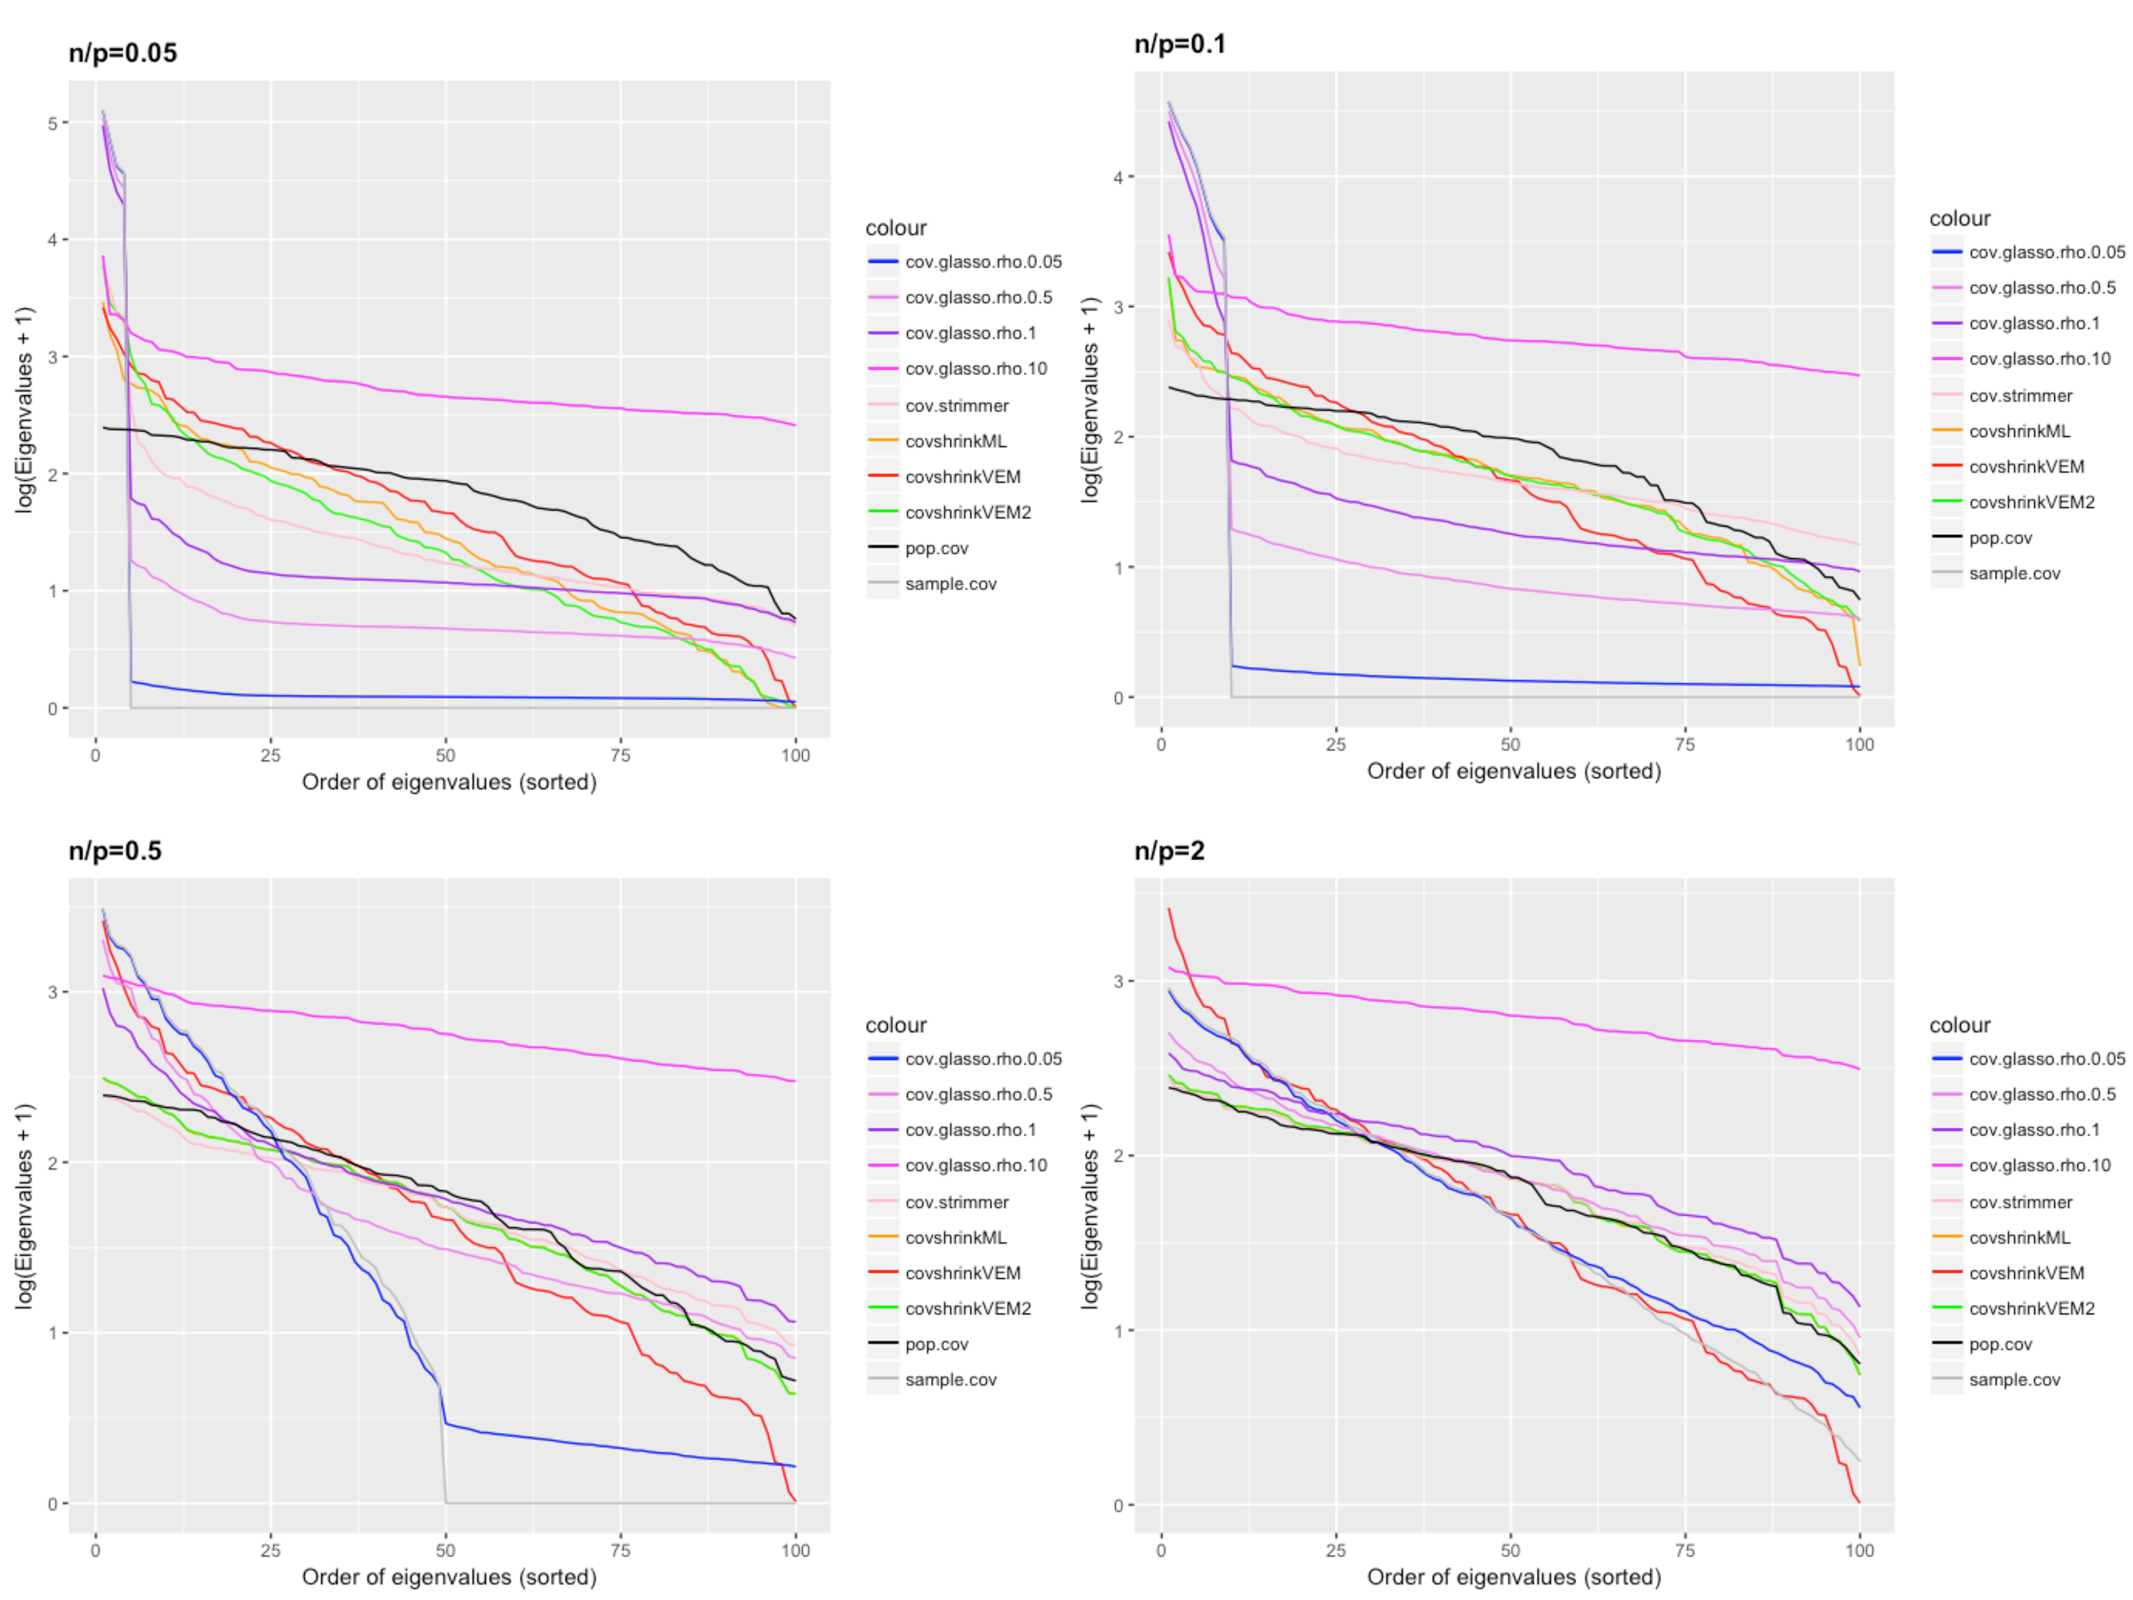
\includegraphics[height=3in, width=6in]{eigenval_dist_2.pdf}
 \caption{Distribution of the sorted eigenvalues for the shrunk covariance matrices due to the three versions of \textit{CorShrink}- namely \textit{CorShrinkML}, \textit{CorShrinkVEM} and \textit{CorShrinkVEM2}, three versions of GLASSO for three regularization parameters $\rho$, varying from $0.05$, $0.5$ and $1$  [ low to high shrinkage ] and the Sch\"{a}fer-Strimmer shrinkage method, along the distributions of the eigenvalues for the sample covariance and the population covariance matrices.}
\label{fig:fig1}
\end{figure*}

Besides the eigenvalue trends and the top few eigenvalues, another important consideration in comparing these shrinkage methods is how close the eigenvectors from the shrunk covariance matrices are with respect to the population covariance matrix. Table ~\ref{tab:tab1} present the average distance between the top 5 eigenvectors of the each shrinkage method with respect to the population covariance. Again we find that the Sch\"{a}fer-Strimmer, \textit{CorShrink-ML} and \textit{CorShrink-VEM2}  produce shrunk covariance matrices closest to the population covariance matrix in terms of the eigen-spaces corresponding to the top eigenvalues. In Figure \ref{fig:fig2}, we plot the distribution of the correlations from the shrunk matrices obtained using different shrinkage methods . We observed that the distribution is more concentrated around $0$ for the  \textit{CorShrink} models when compared to the GLASSO and Sch\"{a}fer-Strimmer methods. Additionally,  \textit{CorShrink} retains some correlation values with large magnitudes. This characteristic of the  \textit{CorShrink} approach would ensure a sparse representation when used in building correlation networks.




\begin{figure*}[ht]
\centering
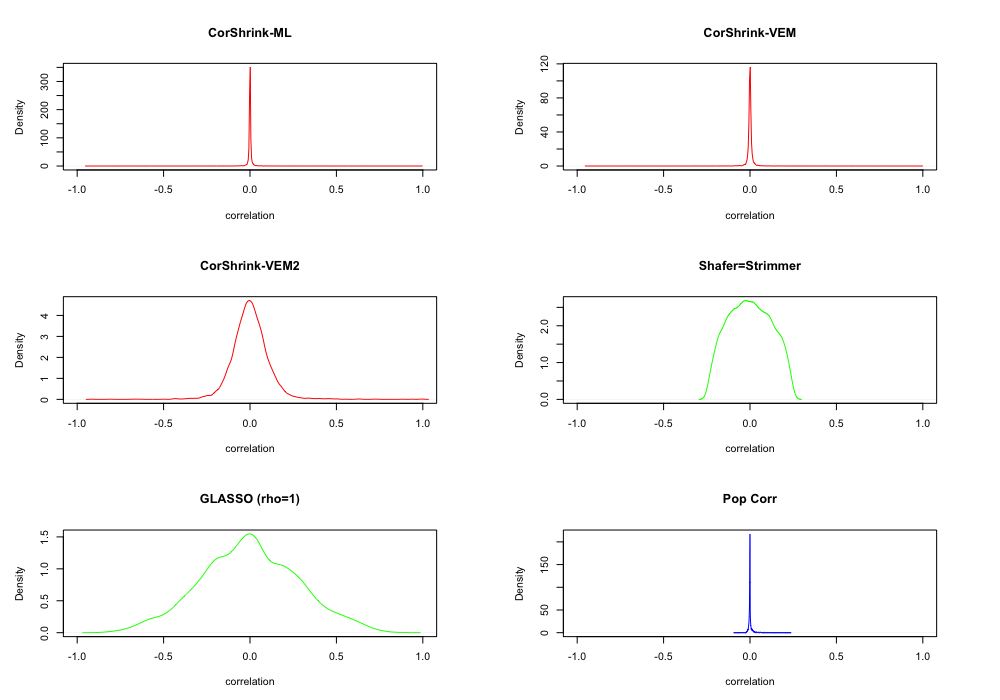
\includegraphics[height=2.5in, width=5in]{correlation_density_compare}
 \caption{Overall distribution of the correlations after shrinking the covariance matrix using the three models of \textit{CorShrink}, Sch\"{a}fer-Strimmer method and the GLASSO method for regularization parameter of $1$ (which was found to be the best fit in terms of eigenvalue patterns out of the four choices considered). The correlation distributions are compared with the actual correlation distribution from the population covariance matrix.}
\label{fig:fig2}
\end{figure*}

\clearpage
\begin{table}[ht]
\begin{center}
\caption{Average Distance of the first 5 eigenvectors of the shrunk covariance matrices from different shrinkage methods versus population covariance matrices. \label{tab:tab2}}
\begin{tabular}{|p{1.5in}|p{0.8in}|p{0.8in}|p{0.8in}|p{0.8in}|}
 \hline
 Methods &  $n/p=0.05$ & $n/p=0.1$ & $n/p=0.5$ & $n/p=2$ \\ \hline
 CorShrink-ML & 0.030 &  0.034  &  0.033  &  0.036 \\ \hline
 CorShrink-VEM  &  0.037  &  0.039  & 0.057  & 0.062 \\ \hline
 CorShrink-VEM2 & 0.031 & 0.046 & 0.043 & 0.037 \\ \hline
 Sch\"{a}fer-Strimmer & 0.037 & 0.054 & 0.051 &  0.044 \\ \hline
 GLASSO ($\rho=0.05$) & 0.083 & 0.085 & 0.085 & 0.069 \\ \hline
 GLASSO ($\rho=0.1$) & 0.078 & 0.083 & 0.084 & 0.061 \\ \hline
 GLASSO ($\rho=0.5$) & 0.064 & 0.081 & 0.081 & 0.057 \\ \hline
 GLASSO ($\rho=1$) & 0.063 & 0.079 & 0.080 & 0.057 \\ \hline
 Sample cov  & 0.083 & 0.084 & 0.085 & 0.076 \\ 
 \hline	
\end{tabular}
\end{center}
 \end{table}
 
 \section{Discussion}
 
Our goal here is to highlight the potential of the \textit{CorShrink} models in performing adaptive correlation and covariance shrinkage that has comparable to better performance over the Sch\"{a}fer Strimmer shrinkage approach in terms of eigen-space and eigenvalue patterns comparisons and that outperforms GLASSO as a correlation shrinkage method irrespective of the choice of regularization parameter used for the latter (see Figure~\ref{fig:fig1} and Table \ref{tab:tab1}).
In terms of computational time, the computation time for the \textit{CorShrink-ML} method is comparable with GLASSO under medium to high shrinkage and Sch\"{a}fer Strimmer method, while \textit{CorShrink-VEM} and \textit{CorShrink-VEM2} are slower in comparison. For instance, the time taken to run \textit{CorShrink-ML}, \textit{CorShrink-VEM} and \textit{CorShrink-VEM2} on the Deng et al samples data were ?? , ??  and ??  seconds whereas that for GLASSO ($\rho =1$) and Sch\"{a}fer-Strimmer methods were ??  . 

The \textit{CorShrink} can be easily extended to partial correlation and partial covariance matrices and also leads to efficient computation of the inverse correlation and covariance matrices. The latter would allow one to build causal networks based on the \textit{CorShrink} models and compare them to the GLASSO based causal networks. An example of a causal network on the samples of the Deng et al data using  the three shrinkage approaches \textit{CorShrink-ML}, Sch\"{a}fer-Strimmer and GLASSO ($\rho=1$) is provided here. This method also opens other areas of applications and extensions that we intend to pursue in future. One can combine Linear Discriminant Analysis and  Multiple regression problem with the shrunk covariance matrices obtained from the \textit{CorShrink} approaches, in the same way the Sch\"{a}fer Strimmer method has been used in these domains \cite{Xu2009} \cite{Schafer2005}. In this paper, we did not consider any additional structure on the covariance matrices. But for structured covariance matrices, one would want to pool the knowledge of the structure into the shrinkage method. For example, for a block covariance matrix, it makes more sense to apply \textit{CorShrink} separately on each block and pool the blocks together. 


The codes to fit the \textit{CorShrink} models on data are implemented in an R package \textbf{CorShrink} which is available on Github at \url{https://github.com/kkdey/CorShrink}. It also contains a README demonstrating how these models could were fitted on simulated data. The Deng et al single cell data \cite{Deng2014} is available as a R data package with instructions for downloading and loading into R at \url{https://github.com/kkdey/singleCellRNASeqMouseDeng2014}.

\begin{thebibliography}{9}

\bibitem{Ledoit2003}
Ledoit O. and Wolf  M. 2003. 
"Improved estimation of the covariance matrix of stock returns with an application to portofolio selection.
\textit{Journal of Empirical Finance}. 10 (5): 603?621.

\bibitem{Ledoit2004}
Ledoit O. and Wolf  M. 2004. 
Honey, I shrunk the sample covariance matrix.
\textit{The Journal of Portfolio Management}. 30 (4): 110?119.

\bibitem{Lancewiki2014}
Lancewicki T. and Aladjem M. 2014.
Multi-Target Shrinkage Estimation for Covariance Matrices.
\textit{IEEE Transactions on Signal Processing}. 62 (24), 6380-6390

\bibitem{Schafer2005}
Sch\"{a}fer J and Strimmer K.  2005. 
A shrinkage approach to large-scale covariance matrix estimation and implications for functional genomics. 
\textit{Statist. Appl. Genet. Mol. Biol}.4.32.

\bibitem{Schafer2005b}
Sch\"{a}fer J and Strimmer K.  2005. 
An empirical Bayes approach to inferring large-scale gene association networks. 
\textit{Bioinformatics}. 21: 754-764.

\bibitem{Stephens2016}
Stephens M. 2016. 
False discovery rates: a new deal. 
\textit{Biostatistics} Advance Access.


\bibitem{Deng2014}
Deng Q,  Ramskold D,  Reinius B,  Sandberg R. 2014.
Single-Cell RNA-Seq Reveals Dynamic, Random Monoallelic Gene Expression in Mammalian Cells.
\textit{Science}.  343 (6167) 193-196.

\bibitem{Xu2009}
Xu P.,  Brock GN,  Parrish RS.  2009.
Modified linear discriminant analysis approaches for classification of high-dimensional microarray data.
\textit{Computational Statistics $\&$ Data Analysis}. 53.5.

\bibitem{Friedman2008}
Friedman J,  Hastie T,  Tibshirani R. 2008.
Sparse inverse covariance estimation with the graphical lasso. 
\textit{Biostatistics}. 9.3.

\bibitem{Witten2010}
Witten DM,  Friedman JH, Simon N. 2010.
New Insights and Faster Computations for the Graphical Lasso. 
\textit{Journal of Computational and Graphical Statistics}, 20, 4, 892?900.

\bibitem{Blei2016}
Blei DM, Kucukelbir A, McAuliffe JD. 2016.
Variational Inference: A Review for Statisticians.
https://arxiv.org/pdf/1601.00670.

\bibitem{Beal2003}
Beal MJ, Ghahramani Z.
The Variational Bayesian EM Algorithm for Incomplete Data: with Application to Scoring Graphical Model Structures
\textit{Bayesian Statistics}, 7.


\end{thebibliography}




\end{document}
